\chapter{Suppression d'un élément dans un arbre binaire de recherche}

\section{Description de l'objectif de l'algorithme}
Les arbres binaires représentent une structure de données très utilisée pour effectuer des tâches en informatique, d’une part parce que ce type de données permet de stocker des données volumineuses facilement accessibles, et d’autre part, les informations sont souvent hiérarchisées, et peuvent être représentées naturellement sous une forme arborescente.
\par
Un arbre est un ensemble organisé de nœuds dans lequel chaque nœud a un seul père, à l’exception de la racine qui est un nœud sans père. 
\par
 Si le nœud p est le père du nœud f, nous dirons que f est un fils de p, et si le nœud p n’a pas de fils nous dirons que c’est une feuille. Chaque nœud porte une valeur (également appelée clé ou étiquette) et deux pointeurs, un qui pointe son fils gauche et l’autre sur le droit.  
 \par
 Un arbre binaire de recherche (ABR) est un arbre qui permet de représenter un ensemble de valeurs ayant une relation d’ordre.C'est à dire que pour tout nœud de cet arbre, sa valeur est strictement plus grande que les valeurs figurant dans son sous-arbre gauche et strictement plus petite que les valeurs figurant dans son sous-arbre droit. Cela implique qu’une valeur n’apparaît au plus qu’une seule fois dans un arbre de recherche.(voir Figure \ref{fig:arb}).
 \par
 Les opérations caractéristiques sur les arbres binaires de recherche sont l’insertion, la suppression, et la recherche d’une valeur. Le cout de ces dernières dépend du degré d’équilibre de l’arbre. 
 \par 
 La suppression d'un élèment dans un arbre binaire de recherche est une opération compliquée. En effet, on doit d'abord trouver le noeud, le supprimer, ensuite nous devons faire le nécessaire pour conserver la structure de l'arbre.  

\begin{figure}[H]
    \centering
        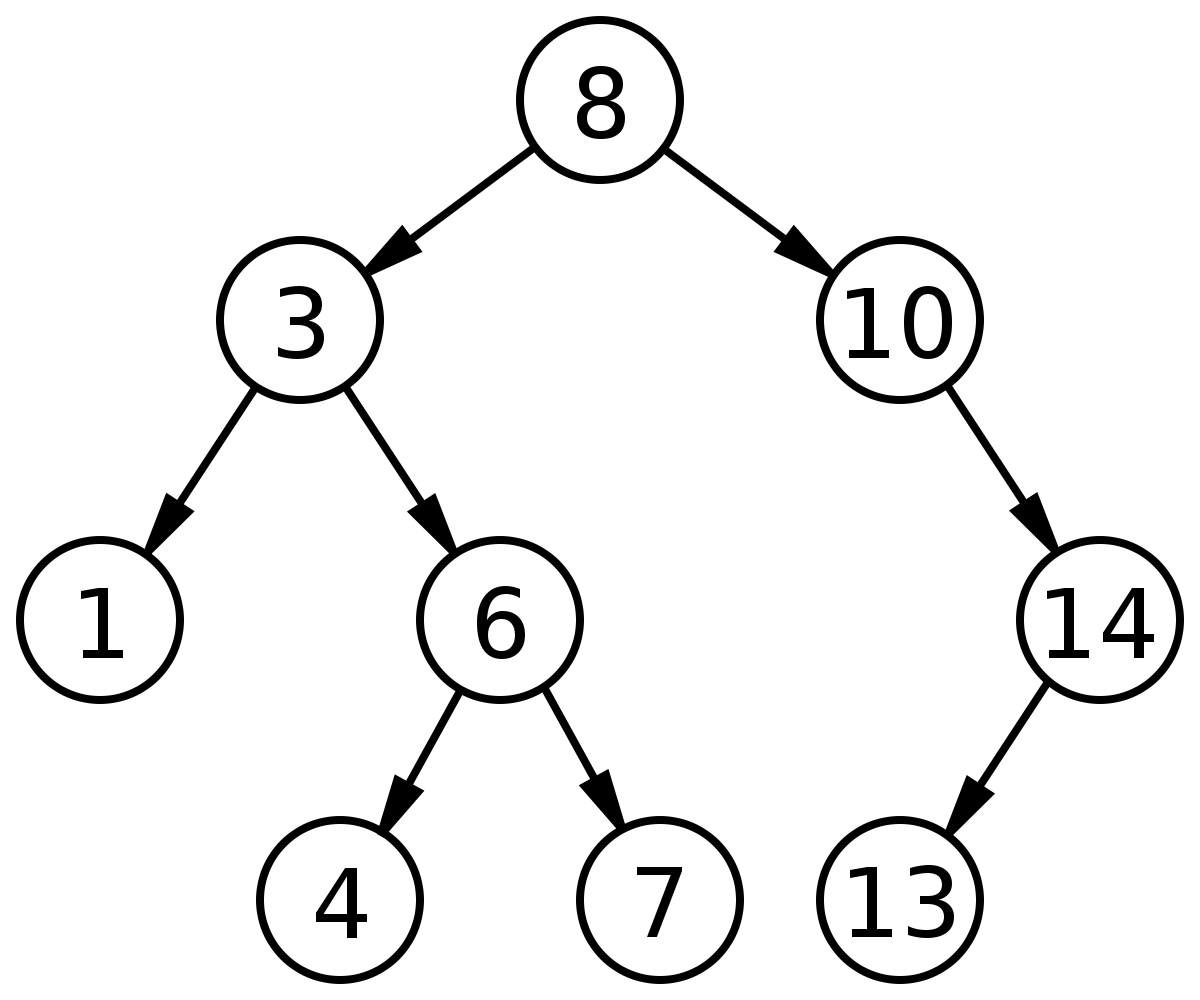
\includegraphics[scale=0.2]{./ressources/arbre.png}
        \caption{Exemple graphique d'un arbre binaire de recherche}
    \label{fig:arb}
\end{figure}

\section{Fonctionnement de l'algorithme}
L’opération de suppression d’un nœud dépend du nombre de ses fils dans l’arbre. Les différents cas de figure possibles sont les suivants

\subsection{Cas 1 : Cas d’une feuille. Le nœud à supprimer n’a pas de fils}
Il suffit d'enlever le nœud en modifiant le lien du père, s’il existe. Sinon l'arbre devient un arbre vide.  (voir Figure \ref{fig:d1}).
\begin{figure}[H]
    \centering
        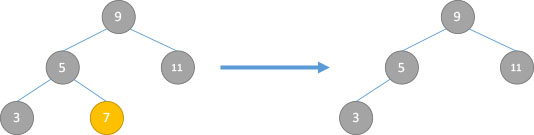
\includegraphics[scale=0.8]{./ressources/d1.jpeg}
        \caption{Exemple de suppression d'une feuille}
    \label{fig:d1}
\end{figure}

\subsection{Cas 2 : Cas d’un unique fils. Le nœud à supprimer à un seul fils}
On décroche le noeud de l’arbre En reliant directement son père et son fils. Ensuite on libère l'espace qu'occupe le noeud à supprimer. Si son père n’existe pas, l’arbre est réduit au fils unique du nœud supprimé.  (voir Figure \ref{fig:d2}).
\begin{figure}[H]
    \centering
        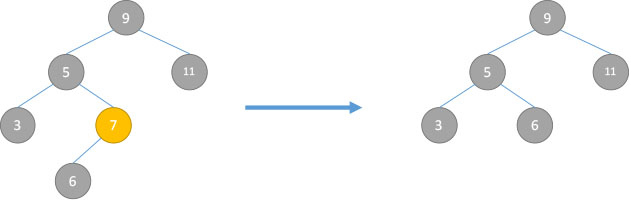
\includegraphics[scale=0.7]{./ressources/d2.jpeg}
        \caption{Exemple de suppression d'un noeud à un seul fils}
    \label{fig:d2}
\end{figure}

\subsection{Cas 3 : Cas de deux fils. Le nœud à supprimer à deux fils}
On cherche le successeur en ordre du noeud. Ensuite, on copie le contenu du successeur d'ordre dans le noeud et on supprime le successeur d'ordre. Notez que le prédécesseur d'ordre peut également être utilisé.
\par
Il est important de noter que le successeur d'ordre peut être obtenu en trouvant la valeur minimale dans le sous-arbre de droite du noeud à supprimer et que le prédécesseur d'ordre est le maximum de son sous-arbre gauche.(voir Figure \ref{fig:d3}).
\begin{figure}[H]
    \centering
        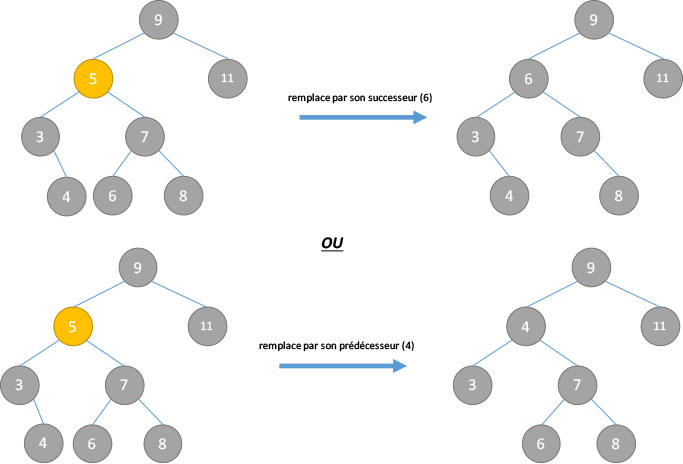
\includegraphics[scale=0.6]{./ressources/d3.jpeg}
        \caption{Exemple de suppression d'un noeud à deux fils}
    \label{fig:d3}
\end{figure}
\par


\begin{function}[H]
\caption{supprimerec(Entrée: racine: arbre, valeur: entier) : arbre}
    \textbf{Variables :}\\
    Temp: arbre\;
    \Begin{
        \If{$racine = Nil$}
            {retour Nil\;}
        \ENDIF
        \If{$valeur < racine.valeur$}{
            \tcp{Si la valeur cherchée est inférieure à l'élèment en cours, on supprime à gauche}
            $racine.filsg \leftarrow supprimerec(racine.filsg, valeur)$\;}
        \ElseIf{$valeur > racine.valeur$}{
        \tcp{Si la valeur cherchée est supérieure à l'élèment en cours, on supprime à droite}
            $racine.filsd \leftarrow supprimerec(racine.filsd, valeur)$\;}
        \Else
        {
        \tcp{Si la valeur est trouvée, on distigue 3 cas}
        \tcp{Le noeud n'a pas de fils}
        \If{$racine.filsg = Nil$ et $racine.filsd = Nil$}{
        retour Nil\;}
        \ElseIf{$racine.filsd = Nil$}
        {
        \tcp{Si le noeud a un fils gauche seulement}
        $Temp \leftarrow racine.filsg$ \;
        Libérer(racine)\;
        retour Temp \;
        }
        \ElseIf{$racine.filsg = Nil$}{
        \tcp{Si le noeud a un fils à droite seulement}
        $Temp \leftarrow racine.filsd$ \;
        Libérer(racine)\;
        retour Temp \;
        }
        
        $Temp \leftarrow Min(racine.filsd)$\; \tcp{Peut etre remplacé par $Temp \leftarrow Max(racine.filsg)$\;}
      }
    }
\end{function}


\begin{function}[H]
\caption{supprimerec(Entrée: racine: arbre, valeur: entier) : arbre}
    \Begin{
        $racine.valeur \leftarrow Temp.valeur$ \;
        $racine.filsd \leftarrow supprimerec(racine.filsd, Temp.valeur)$ \; \tcp{Peut etre remplacé par $racine.filsg \leftarrow supprimerec(racine.filsg, Temp.valeur)$ \;}
        retour racine;
        }
    
\end{function}


\singlespacing
\par 
Comme nous l'avons mentionné avant, quand on veut supprimer un nœud qui a deux fils, nous devons écraser sa valeur en optant pour l’une des deux options : soit on cherche le successeur en ordre du nœud à supprimer, soit son prédécesseur en ordre. Il est à noter que le successeur en ordre du nœud représente le minimum dans son sous-arbre à droite, et que son prédécesseur représente le maximum de son sous-arbre gauche. Voici donc les deux fonctions que nous pourrons utiliser pour effectuer ces deux tâches :
\singlespacing
\begin{function}[H]
    \textbf{Variables :}\\
    min: arbre\;
    \Begin{
    $min \leftarrow racine$ \;
        \While{$min <> Nil$ et $min.filsg <> Nil$}{
        $ min \leftarrow min.filsg$ \;
       }
       retour min;
    }
    \caption{Min(Entrée: racine: arbre) : arbre}
\end{function}

\begin{function}[H]
    \textbf{Variables :}\\
    max: arbre\;
    \Begin{
    $max \leftarrow racine$ \;
        \While{$max <> Nil$ et $max.filsd <> Nil$}{
        $ max \leftarrow max.filsd$ \;
       }
       retour max;
    }
    \caption{Max(Entrée: racine: arbre) : arbre}
\end{function}
\singlespacing
\par 
Puisque l’opération de suppression est une tâche complexe, nous avons, en premier lieu opter pour la méthode récursive. Celle-ci nous permet d’avoir une vue globale sur les cas auxquels nous pourrons être confrontés et comment procéder pour garder la structure de l’arbre intacte même après la suppression.  
\par
Maintenant, nous allons écrire l’algorithme itératif de suppression pour comprendre comment s’effectue la suppression en détail. 

\begin{function}[H]
    \textbf{Variables :}\\
    inter, actuel, min, pere : arbre\;
    \Begin{
    $actuel \leftarrow racine$ \;
    $pere \leftarrow Nil$ \;
        \While{$actuel <> Nil$ et $actuel.valeur <> valeur$}{
        $ pere \leftarrow actuel$ \;
        \If{valeur < actuel.valeur}{
        $actuel \leftarrow actuel.filsg$\;
        \Else{$actuel \leftarrow actuel.filsd$\;}
        }
        }
        \If{$actuel = Nil$}{
        Ecrire("La valeur que vous voulez supprimer n'existe pas dans l'arbre")\;
        retour Nil\;
        }
        \If{$actuel.filsg = Nil$ ou $actuel.filsd = Nil$}{ \tcp{Si le noeud a au plus un fils}
        \If{$actuel.filsg = Nil$}{ 
        $inter \leftarrow actuel.filsd$\;
        }
        \Else{$inter \leftarrow actuel.filsg$\;}
        \If{$pere = Nil$}{ \tcp{Si le noeud est une racine}
        retour inter\;
        }
        \If{actuel = pere.filsd}{ \tcp{Si le noeud est une fils à droite}
        pere.filsd = inter\;
        }
        \Else{pere.filsg = inter\;}
        Libérer(actuel)\;
        }
    }
    \caption{supprimeiter(Entrée: racine: arbre, valeur: entier) : arbre}
\end{function}



\begin{function}[H]
\caption{supprimeiter(Entrée: racine: arbre, valeur: entier) : arbre}
     \Else{ \tcp{Si le noeud à supprimer a deux fils}
        \tcp{On commence par chercher le successeur en ordre}
        $min \leftarrow actuel.filsd$\;
        $pere \leftarrow racine$\;
        \While{$min.filsg <> Nil$}{
        $pere \leftarrow min$\;
        $min \leftarrow min.filsg$\;
        }
        \If{$pere <> racine$}{
        \tcp{On peut mettre fils droit du successeur comme fils gauche du père du successeur }
        $pere.filsg \leftarrow min.filsd$\;
        }
        \Else{
        $actuel.filsd \leftarrow min.filsd$\;
        }
        $actuel.valeur \leftarrow min.valeur$\; \\
        Libérer(min)\;
        }
        retour racine\;
        FIN.
\end{function}


\section{Calcul de complexité}
\subsection{Complexité temporelle}
Dans le meilleur cas, nous aurons un ABR équilibré, c’est-à-dire que le nombre des fils à gauche est le même qu’à la droite. Ainsi, l'opération de se fera que sur la motié de l'ABR équilibre, ce qui donne une complexité de $\mathcal{O}(log_2(n))$.  
\par
Nous avons obtenu une complexité temporelle logarithmique parce que la suppression dans un arbre binaire de recherche est un cas où un problème de taille n est divisé en sous-problèmes de taille n/2 jusqu'à atteindre un problème de taille 1.
\par
Le calcul de la complexité se fait donc de la manière suivante :
$$ \frac {a}{b^x}=1  \hspace{2cm}[Dans\hspace{0.2cm} un\hspace{0.2cm} arbre\hspace{0.2cm} binaire\hspace{0.2cm} b = 2] $$
$$i.e : n=2^x\hspace{2cm} qui\hspace{0.2cm} est\hspace{0.2cm} log_2 n\hspace{0.2cm} par\hspace{0.2cm} definition\hspace{0.2cm} de\hspace{0.2cm} la\hspace{0.2cm} fonction\hspace{0.2cm} logarithme$$
\par 
Dans le cas moyen, la complexité temporelle est de l’ordre de la hauteur de l’arbre binaire de recherche. Puisque ce dernier est en moyenne $\mathcal{O}(log_2(n))$, la complexité temporelle du cas moyen est de l’ordre $\mathcal{O}(log_2(n))$.
\par
Par ailleurs, si on traverse de la racine à une feuille, c’est-à-dire toute la hauteur $h$ de l’arbre. Si ce dernier n’est pas équilibré, on sera amené à parcourir tous les nœuds et la hauteur de l’arbre deviendra $n$. par conséquent la complexité temporelle dans le pire des cas de l’opération de suppression est $\mathcal{O}(n)$.
\par
La complexité temporelle de la suppression d’un nœud ne diffère pas grandement entre l’approche récursive et l’itérative étant donné que chaque boucle dans cette dernière est remplacée par un appel récursif de la fonction dans la deuxième approche.
\par
Dans la suppression itérative, on commence d’abord par chercher la valeur à supprimer en utilisant une boucle à n itérations. Ensuite une fois trouvée, si le nœud contenant cette valeur a deux fils, nous devons une fois de plus faire la recherche du minimum (resp. Maximum) dans son sous arbre à droite (resp. Gauche) qui contient $n’$ éléments.
\par
Dans le meilleur et moyen cas, l’arbre sera complètement équilibré et donc la complexité temporelle sera $\mathcal{O}(log_2(n - n') +log_2(n')) \approx  \mathcal{O}(log_2(n))$.
\par
Dans le pire cas la complexité sera $\mathcal{O}((n -n')) + {O}(n') \approx  {O}(n)$. 
\par
Dans la suppression récursive, on compare à chaque fois la valeur cherchée avec la valeur en cours et on effectue des appels récursifs jusqu’à trouver la valeur voulue. Ensuite, si le nœud contenant cette valeur a deux fils, nous devons faire la recherche du minimum (resp. Maximum) dans son sous arbre à droite (resp. Gauche) afin d’écraser sa valeur. Finalement, on effectue un autre appel récursif sur le même sous-arbre pour supprimer la valeur du minimum.
\par
Dans le meilleur et moyen cas, l’arbre sera complètement équilibré et donc la complexité temporelle sera  $\mathcal{O}(log_2(n - n') +log_2(n')) + \mathcal{O}(n'/2) \approx \mathcal{O}(n)$
\par 
Dans le pire cas la complexité sera $\mathcal{O}((n -n')) + {O}(n') + {O}(n'/2) \approx {O}(n)$

\par
Le tableau suivant représente les temps d'exécution théorique en nanoseconde de l'algorithme de suppression de la racine selon la variation de la taille de l'arbre.

\small
\begin{center}
\begin{tabular}{| c | c | c | c | c | c | c | c | c | c | c | c | c |}
    \hline
    N &  10 & 50 & 100 & 500 & 1000 & 5000 & 10000 & 100000 & 1000000 & 10000000 \\
    \hline
    t(ns) & 490 & 560 & 720 & 830 & 1130 & 1280 & 1380 & 1590 &  2489 & 2680  \\
    
    \hline
\end{tabular}  
\end{center}

La figure suivante (voir Figure \ref{fig:temps_exec_abr_theo}) représente l'évolution du temps d'exécution théorique selon la taille de l'arbre binaire de recherche.

\begin{figure}[H]
    \centering
        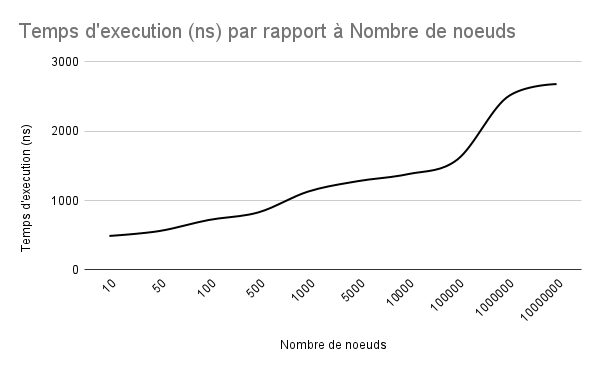
\includegraphics[scale=0.7]{./ressources/exe theo.png}
        \caption{Temps d'exécution théorique du programme selon la taille de l'arbre}
    \label{fig:temps_exec_abr_theo}
\end{figure} 

Depuis le graphe,  on observe que le temps d'exécution évolue de manière linéarithmique avec l'augmentation de la taille du problème.

\subsection{Complexité spatiale}

\par
Nos noeuds sont directement stockées dans un arbre de recherche à $n$ éléments. Dans notre cas, un noeud contient une valeur entière et deux pointeurs pour les deux fils. La taille de la valeur stockée ainsi que celle d'un pointeur fait 4 octets. Donc la taille d'un élèment dans l'arbre est égale à $4+ 4*2$ unités donc $12$ unités.
\par
La complexité spatiale de l’algorithme est $\mathcal{O}(n)$.
\par

\section{Expérimentation}
Le tableau suivant représente les temps d'exécution en nanoseconde de l'algorithme de suppression dans un arbre à 10 noeuds selon l'approche utilisée, l'équillibre de l'arbre et le nombre de fils du noeud à supprimer.\\ 
\singlespacing
\small
\resizebox{17cm}{!}{
\begin{tabular}{| c | c | c | c | c |}
    \hline
    Type d'approche & Type d'arbre & Type de Suppression &  Temps d'execution (ns) \\
    \hline
    \multirow{9}*{Récursive} & \multirow{3}*{Arbre partiellement équilibré}  &  noeud avec deux fils & 1651\\
    \cline{3-4}
      &   &  noeud avec un fils & 1960 \\
    \cline{3-4}
      &  &  noeud feuille & 1080 \\
    \cline{2-4}
      & \multirow{3}*{Arbre complétement équilibré}  &  noeud avec deux fils & 290\\
    \cline{3-4}
      & &  noeud avec un fils & 280\\
    \cline{3-4}
      &   &  noeud feuille & 220\\
    \cline{2-4}
      & \multirow{3}*{Arbre complétement Déséquilibré} &  noeud avec deux fils & 290 \\
    \cline{3-4}
      &  &  noeud avec un fils & 290\\
    \cline{3-4}
      &  &  noeud feuille & 230 \\
    \hline
    \multirow{9}*{Itérative} & \multirow{3}*{Arbre partiellement équilibré}  &  noeud avec deux fils & 160 \\
    \cline{3-4}
      &  &  noeud avec un fils & 300 \\
    \cline{3-4}
      & &  noeud feuille & 410\\
    \cline{2-4}
      & \multirow{3}*{Arbre complétement équilibré} &  noeud avec deux fils & 260 \\
    \cline{3-4}
      &  &  noeud avec un fils & 200\\
    \cline{3-4}
      &  &  noeud feuille & 160\\
    \cline{2-4}
      & \multirow{3}*{Arbre complétement Déséquilibré}  &  noeud avec deux fils & 250\\
    \cline{3-4}
      &  &  noeud avec un fils & 280 \\
    \cline{3-4}
      &  &  noeud feuille & 200 \\
    \hline
\end{tabular}}
\singlespacing
\par
En effet, nous constatons du tableau que l’algorithme itératif est toujours plus rapide que le récursif. Par ailleurs, la complexité temporelle de la suppression augmente selon le nombre de fils du nœud à supprimer. Plus il a de fils, plus le temps d’exécution est élevé.\\ 
\par
Le tableau suivant représente les temps d'exécution en nanoseconde de l'algorithme de suppression de la feuille la plus lointaine de la racine dans un arbre quelconque en utilisant une approche itérative.\\ 
\singlespacing
\small
\resizebox{17cm}{!}{
\begin{tabular}{| c | c | c | c | c | c | c | c | c | c | c | c | c |}
    \hline
    N &  10 & 50 & 100 & 500 & 1000 & 5000 & 10000 & 100000 & 1000000 & 10000000 \\
    \hline
    t1(ns) & 540 & 691 & 610 & 960 & 910 & 1251 & 1980 & 1581 & 6980 & 8430 \\
    \hline
    t2(ns) & 300 & 220 & 450 & 690 & 880 & 960 & 1350 & 2250 & 6961 & 11260 \\
    \hline
    t3(ns) & 210 & 260 & 470 & 980 & 780 & 920 & 1900 & 2420 & 6611 & 10610 \\
    \hline
    t4(ns) & 200 & 230 & 680 & 1160 & 740 & 950 & 1160 & 4460 & 6971 & 8520 \\
    \hline
    t5(ns) & 200 & 290 & 340 & 610 & 1040 & 1010 & 2049 & 3331 & 5601 & 9040 \\
    \hline
    t6(ns) & 270 & 200 & 300 & 690 & 550 & 1220 & 1250 & 3810 & 6140 & 9061 \\
    \hline
    t7(ns) & 330 & 250 & 361 & 580 & 690 & 1170 & 1380 & 3680 & 6690 & 12340 \\
    \hline
    t8(ns) & 250 & 310 & 279 & 670 & 980 & 819 & 1310 & 1720 & 6430 & 8790 \\
    \hline
    t9(ns) & 230 & 450 & 290 & 650 & 840  & 820 & 1450 & 2291 & 6191 & 7999 \\
    \hline
    t10 (ns) & 210 & 681 & 310 & 779 & 760 & 960 & 1520 & 2690 & 6399 & 9900 \\
    \hline
    Moyenne (ns) & 274 & 358 & 409 & 776 & 817 & 1008 & 1534 & 2823 & 6497 & 9595 \\
    \hline
\end{tabular}
}
\singlespacing
\normalsize
\par
La figure suivante (voir Figure \ref{fig:temps_exec_noeuds}) représente l'évolution du temps d'exécution selon la taille de l'arbre.

\begin{figure}[H]
    \centering
        \includegraphics[scale=0.7]{./ressources/Temps d'execution (ns) par rapport à Nombre de noeuds .png}
        \caption{Temps d'exécution du programme selon le nombre de noeuds}
    \label{fig:temps_exec_noeuds}
\end{figure}
\par
Depuis le graphe, la courbe est sous forme de courbe ascendante, on observe que le temps d'exécution évolue avec l'augmentation de la taille du problème, ce qui correspond bien à la complexité théorique calculée auparavant. 

\section{Conclusion}
La suppression d’un nœud dans un arbre binaire de recherche est l’une des opérations les plus compliquées à faire étant donné qu’il faut appliquer un traitement différent selon le nombre de fils que le nœud à supprimer possède.  Dans cette partie, nous avons essayé les deux approches : itérative et récursive. Nous constatons qu’en utilisant cette dernière, le code est plutot petit et facile à comprendre contrairement à la façon itérative qui est beaucoup plus lourde.En revanche, cette dernière nous aide à comprendre de manière détaillée tout ce qui se passe en interne dans l'algorithme et comment la suppression est réellement effectuée.De plus, elle est plus rapide que l'approche récursive.